\section{Bildverarbeitung}
\label{sec:bildverarbeitung}

Weil das Zielfeld im Gegensatz zum Holzwürfel nicht an einer vorher definierten Stelle auf der x-Achse zu liegen kommt, muss dieses optisch erkannt werden. Hierzu wird, wie in PREN 1 \cite[S. 25-26]{pren1} beschrieben, die Raspi-Cam zusammen mit der Bildverarbeitungsbibliothek OpenCV und der Programmiersprache Python 3 verwendet. Die Herausforderung besteht nicht nur in der Erkennung des Zielfeldes, sondern auch in der Ermittlung der jeweils gegenwärtigen Distanz der Last zum Zielfeld.

\subsection{Lösungsansatz}
\label{sec:loesungsansatz}

Wird die Kamera nach unten zeigend parallel zur Unterlage ausgerichtet, ist der Bildmittelpunkt direkt unterhalb der Kameralinse. Die Distanz von der Kameralinse zum Lastmittelpunkt kann anhand der CAD-Pläne auf ca. $11cm$ festgelegt werden. Dies ist die Distanz, welche die Kamera über das Ziel hinweg positioniert werden muss, um die Last möglichst in der Mitte des Zielfeldes abzulegen.

Die Seitenlänge des innersten Zielfeldquadrates ist in der Aufgabenstellung mit $6cm$ definiert. Dies ist ein wichtiger Referenzwert, anhand dessen der horizontale Abstand zwischen Kameralinse und Zielfeldmittelpunkt ermittelt werden kann.

Die Kamera kann die Seitenlänge des innersten Zielfeldes sowie den Abstand von Bildmitte zum Mittelpunkt des innersten Zielfeldes \textit{in Pixeln} ermitteln. Mit dem Bruch $\frac{\text{ZielfeldhöhePixel}}{6cm}$ kann ermittelt werden, wie vielen Pixeln ein Zentimeter auf dem Bild entspricht. Der horizontale Abstand zwischen Kameralinse und Zielfeldmittelpunkt kann so von Pixeln in eine Distanz in Zentimetern umgerechnet werden.

Dieser Lösungsansatz stellt besondere Anforderungen an die Konstruktion:

\begin{enumerate}
    \item Die Sicht der Kamera nach unten und vorne darf durch kein Bauteil versperrt werden.
    \item Die Kamera muss möglichst parallel zum Untergrund ausgerichtet sein. Seitliche Schwingungen sind unproblematisch, solange das Zielfeld im Sichtfeld bleibt. Starke Schwingungen nach vorne und hinten hingegen lassen das Zielfeld optisch über die gedachte horizontale Bildmittellinie springen, wodurch der hier ausgearbeitete Lösungsansatz nicht mehr funktionieren würde.
\end{enumerate}

Die erarbeitete mechanische Konstruktion erfüllt diese beiden Anforderungen. (Einzig der Blick nach hinten ist von der Greifeinheit versperrt, wodurch zur genauen Positionierung über dem Zielfeld auf den Ultraschallsensor zurückgegriffen werden muss.)

\subsection{Umsetzung}

Die Python-Klasse \texttt{ImageAnalyzer} verfügt über eine Methode namens \texttt{calculate\_distance}, welche von aussen aufzurufen ist. Diese erwartet als Parameter ein Bild als NumPy-Matrix im BGR-Farbraum. Das Bild wird zunächst in Graustufen umgewandelt, indem alle Bildpunkte abhängig von ihrem Helligkeitswert schwarz oder weiss eingefärbt werden.\footnote{Das Zielfeld ist schwarz-grau und nicht schwarz-weiss. In der Praxis trifft man kaum auf ein reines Schwarz oder Weiss.} Das Verfahren wird in \appref{app:thresholding} beschrieben. So wird verhindert, dass feine Linien und Verunreinigungen sowie Klebebänder nicht als Kanten erkannt werden, sondern gleich verschwinden.

Die Polygon-Konturen auf einem Bild können mit der OpenCV-Funktion \texttt{findContours} ermittelt werden. Diese gibt neben einer Liste von Konturmatrizen -- bestehend aus den Koordinaten der Polygonknoten -- die dazugehörigen Polygonhierarchieen zurück. Letztere gibt Auskunft über die Verschachtelungen der ermittelten Polygone.\footnote{Ein Eltern-Polygon beinhaltet ein Kind-Polygon vollständig. Benachbarte Polygone schneiden einander nicht. Das äusserste Polygon einer Hierarchie hat kein Elternpolygon, das innerste Polygon hat kein Kindpolygon.}

Die so ermittelten Polygone müssen genauer untersucht werden, denn es es werden bei weitem mehr gefunden als bloss die konzentrischen Quadrate des Zielfeldes: etwa die gezackten Hindernisse in Form von Tannenattrappen oder die Holzplatten der Unterlage. Diese sollen nach dem Ausschlussverfahren eliminiert werden, indem folgende Heuristiken zum Einsatz kommen:

\begin{description}
    \item[Benachbarte Polygone] Liegen zwei Polygone nebeneinander, bezeichnet man diese als benachbart. Das Zielfeld ist eine Hierarchie von Polygonen, und nur das äusserste Quadrat kann so plausiblerweise einen (oder mehrere) Nachbarn haben. Ein Polygon, das einen Nachbarn hat, ist kein inneres Quadrat des Zielfeldes und kann somit ausgeschlossen werden.
    \item [Quadratische Form] Die zu ermittelnden Polygone sind auf dem Bild nahezu quadratisch, wobei durch perspektivische Verzerrung und Verschwimmen des Bildes (wegen Bewegungsunschärfe) niemals perfekt quadratische Polygone gefunden werden können. Es genügt jedoch Polygone, die nicht einmal näherungsweise ein Quadrat darstellen können, aufgrund zweier Kriterien auszuchliessen:
        \begin{enumerate}
            \item \textsc{Anzahl Ecken}: Ein Quadrat hat vier Ecken. Ein Hindernis, wie die grüne Tannenattrappe ungefähr zwanzig. Polygone mit einer von vier abweichenden Anzahl Knoten können ausgeschlossen werden.
            \item \textsc{Verhältnis Höhe/Breite}: Bei einem Quadrat ist die Höhe gleich der Breite. Bei einem nahezu quadratischen Polygon sollte das Verhältnis $\frac{\text{Höhe}}{\text{Breite}}$ im Bereich $[0.75..1.25]$\footnote{Diese Werte wurden bei Versuchen ermittelt und funktionierten zuverlässig.} liegen.
        \end{enumerate}
    \item[Absolute Grösse] Das innerste Quadrat des Zielfeldes nahm bei Tests immer mehr als 0.5\% der gesamten Bildfläche ein. Das äusserste Quadrat war niemals grösser als 95\% der Bildfläche. Polygone, deren Grösse nicht in dieses Fenster fällt, können ausgeschlossen werden.\footnote{Je nach konfigurierter Vorder- und Hintergrundfarbe kann der Bildrand als Polygon erkannt werden. Die Fläche dieses Polygons beträgt dann 100\% der Bildgrösse.}
\end{description}

Nachdem die Anzahl der gefundenen Polygone nach dem beschriebenen Heuristik-Au\-sschluss\-ver\-fahren reduziert worden ist, bleibt eine Liste von \textit{Kandidaten} übrig, die möglicherweise ein Zielfeld darstellen. Nun gilt es, diese Kandidaten genauer zu untersuchen. Hierzu wird wiederum die Polygonhierarchie verwendet, die schon bei der Ermittlung benachbarter Polygone hilfreich war.

\subsubsection{Die Polygonhierarchie}

Die bereits erwähnte OpenCV-Funktion \texttt{findContours} gibt neben den Polygonkoordinaten auch für jedes Polygon eine Liste bestehend aus vier Zahlen zurück. Die ersten beiden Zahlen handeln von der Nachbarschaftsbeziehung und sind Referenzen auf den Index des vorhergehenden bzw. des nachfolgenden Nachbarpolygons. Da sich in der gefilterten Kandidatenliste keine Polygone mit Nachbarn mehr befinden, können diese Angaben ignoriert werden.\footnote{Sie haben allesamt den Wert \texttt{-1}. Das bedeutet: Kein Nachbar vorhanden.}

Die dritte Zahl gibt den Index des ersten Kindpolygons an. (Da Polygone mit Nachbarn nicht in der Liste vorkommen, gibt es immer nur ein Kindpolygon.) Die vierte Zahl gibt den Index des Elternpolygons an.\footnote{Die Hierarchie-Liste mit vier Elementen ist also als Knoten von gleich zwei verketteten Listen zu verstehen: Einerseits als Element der Nachbarschaftskette und andererseits als Element der Eltern-Kind-Beziehungskette.}

Gesucht ist das \textit{innerste Zielfeld}. Dieses ist definiert als ein Quadrat, das von einem anderen Quadrat umschlossen wird, aber selber keine weiteren Quadrate enthält. Übersetzt auf die Hierarchie-Liste bedeutet das also, dass das dritte Element (erstes Kindpolygon) auf kein anderes Polygon verweisen darf (Wert: \texttt{-1}) und das vierte Element (Elternpolygon) einen gültigen Wert haben muss (Konturindex des jeweiligen Elternpolygons). Wird ein solches Quadrat gefunden, das zuvor schon durch verschiedene Heuristikprüfungen gekommen ist, wird dieses als das innerste Feld des Zielfeldes angenommen. Der Mittelpunkt dieses Polygons wird über die OpenCV-Funktion \texttt{moments} ermittelt.

Wie bereits weiter vorne beschrieben (\secref{sec:loesungsansatz}) kann nun der Abstand zu diesem Zielfeld errechnet werden. Die genaue Positionierung der Last über dem Zielfeld ist im Abschnitt \secrefplain{sec:ablauf} beschrieben.

\subsubsection{Abwägungen}

Die Ermittlung des innersten Zielfeldes könnte noch etwas solider umgesetzt werden, indem nicht nur geprüft wird, ob das innerste Zielfeld \textit{ein} Elternpolygon hat, sondern indem eine \textit{rekursive} Prüfung vorgenommen würde. Das Elternpolygon des innersten Zielfeldes hat wiederum ein Elternpolygon, welches wiederum ein Elternpolygon hat usw. Das vorliegende Zielfeld besteht aus sechs konzentrischen Quadraten, das innerste Zielfeld müsste also fünf übergeordnete Hierarchiestufen besitzen -- und nicht bloss eine. Eine rekursive Prüfung wäre somit solider.

Andererseits bringt eine rekursive Prüfung auch Probleme mit sich:

\begin{description}
    \item[Implementierung] Eine rekursive Prüfung ist aufwändiger umzusetzen und somit fehleranfälliger. Es besteht die Gefahr für Endlosschleifen und somit für einen Stack Overflow, der das Programm zum Abstürzen bringen würde. Das Problem ist zugegebenermassen nicht schwierig zu lösen, und die Endlosschleife könnte mittels Heuristiken vermieden werden. Die Codemenge und -komplexität würde dennoch zunehmen -- und damit auch die Fehlerwahrscheinlichkeit.
    \item[Anzahl Hierarchiestufen] \imgrefplain{fig:zielfeld5} und \imgrefplain{fig:zielfeld6} zeigen das Zielfeld während zweier kurz aufeinanderfolgenden Phasen der Überfahrt. Einmal werden die äusseren beiden Quadrate erkannt, einmal nicht. Dies hat wohl damit zu tun, dass die feine weisse Linie zur Ausrichtung des Zielfeldes auf der x-Achse auf dem etwas verschwommenen Bild den Eindruck macht durchgezogen zu sein. Optisch können keine Quadrate sondern nur halbierte Quadrate (eine andere Art von Polygon mit acht statt vier Ecken) erkannt werden. Die Anzahl der zu prüfenden Hierarchiestufen kann also nicht mit absoluter Sicherheit angegeben werden.
    \item[Früherkennung] Diese beiden genannten Probleme sind sind eher Erschwernisse und Einschränkungen und sollten kein Hindernis für die Umsetzung der rekursiven Hierarchieprüfung darstellen. Aus Gründen der Performance ist die Hierarchieprüfung aber ein grosses Problem. Hierbei geht es nicht etwa um die Programmlaufzeit, sondern um den Zeitpunkt, ab dem das Zielfeld zum ersten mal erkannt werden kann. Ein Blick auf die Bildserie (Seite \pageref{fig:bildserie}) führt dies vor Augen: Auf dem ersten Bild wird noch kein Zielfeld erkannt, da noch kein Quadrat vollständig auf dem Bild sichtbar ist. Auf dem zweiten Bild wird ein Quadrat erkannt.\footnote{Die Bildserie stammt von einem frühen Prototyp der Bildverarbeitung, die alle erkannten Quadrate markiert hat. Mit der Hierarchieprüfung dürfte auf dem zweiten Bild noch kein Zielfeld erkannt werden.} Auf dem dritten Bild werden bereits drei Quadrate erkannt, auf dem vierte Bild sind es bereits fünf Quadrate. Sechs Quadrate werden zum ersten mal auf dem fünften Bild erkannt. Würde die Hierarchie rekursiv geprüft, würde das Zielfeld nicht zum ersten mal mit einem Abstand von $23.4cm$ (\imgrefplain{fig:zielfeld3}) sondern erst mit einem Abstand von $16.3cm$ (\imgrefplain{fig:zielfeld5}) erkannt. \textit{Je tiefer die zu prüfende Hierarchie gewählt wird, desto später wird das Zielfeld erkannt.}
\end{description}

Aus diesen genannten Gründen wurde auf eine \textit{rekursive} Hierarchieprüfung verzichtet. Bei Tests ist bisher nie ein falsches Zielfeld erkannt worden. Die Probleme bestanden eher darin, dass zu Beginn bestimmte Parameter zu streng definiert waren, was später etwas gelockert wurde.

\begin{figure}
    \centering
    \begin{subfigure}{0.3\textwidth}
        \centering
        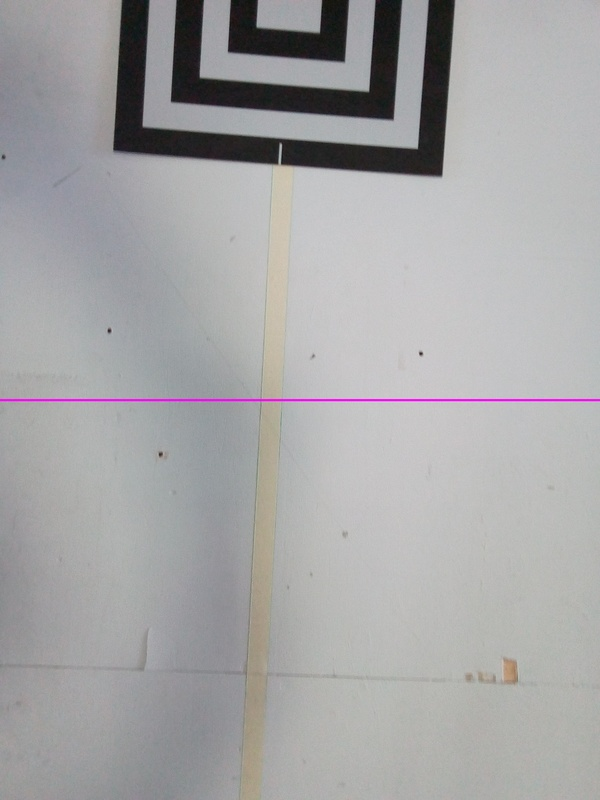
\includegraphics[width=0.95\linewidth]{pics/zielfeld/01.jpg}
        \caption{noch nichts erkannt}
        \label{fig:zielfeld1}
    \end{subfigure}
    \begin{subfigure}{0.3\textwidth}
        \centering
        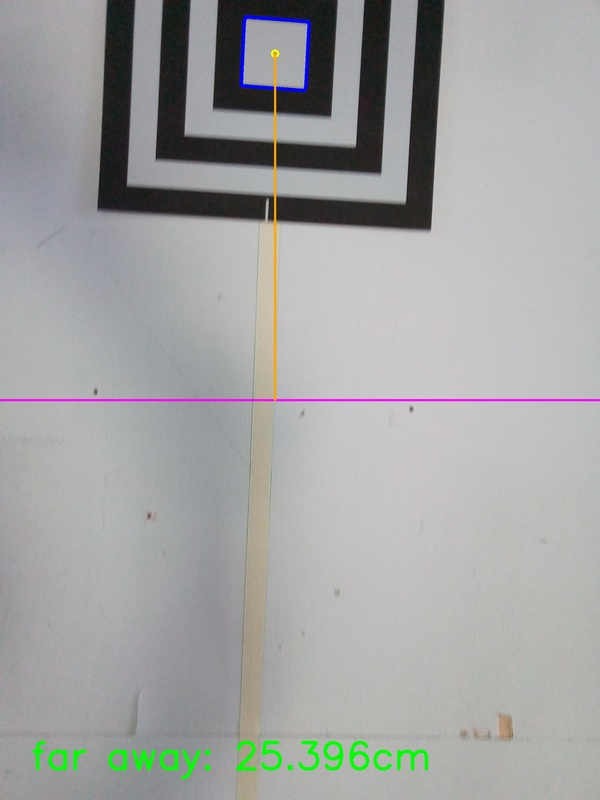
\includegraphics[width=0.95\linewidth]{pics/zielfeld/02.jpg}
        \caption{erstes Quadrat}
        \label{fig:zielfeld2}
    \end{subfigure}
    \begin{subfigure}{0.3\textwidth}
        \centering
        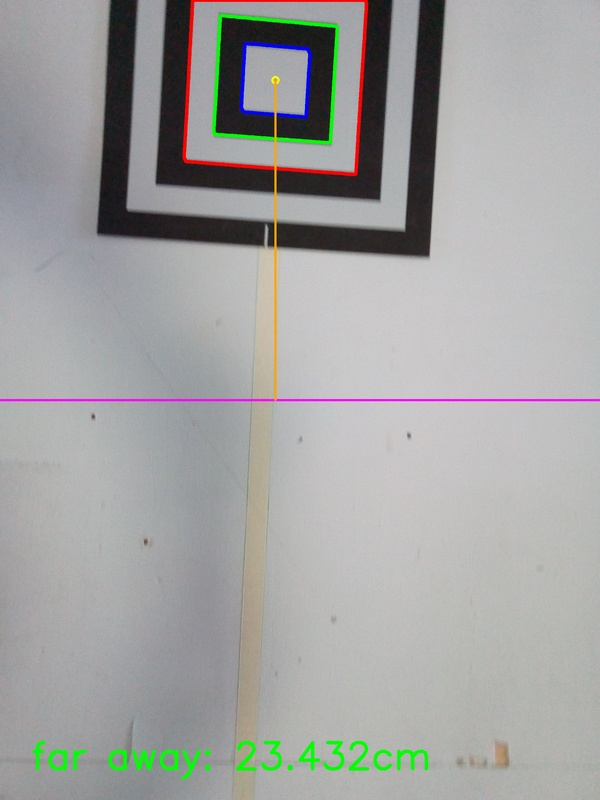
\includegraphics[width=0.95\linewidth]{pics/zielfeld/03.jpg}
        \caption{weitere Quadrate}
        \label{fig:zielfeld3}
    \end{subfigure}
    \vskip\baselineskip
    \begin{subfigure}{0.3\textwidth}
        \centering
        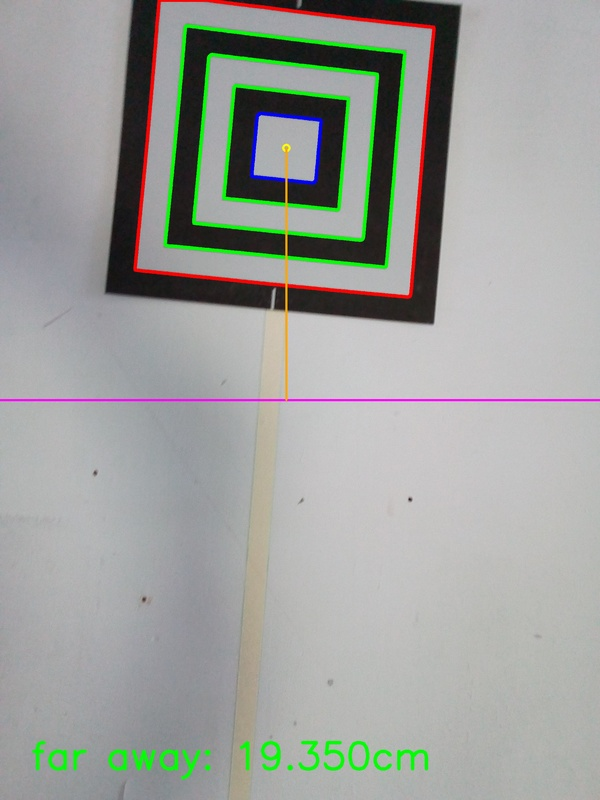
\includegraphics[width=0.95\linewidth]{pics/zielfeld/04.jpg}
        \caption{noch mehr Quadrate}
        \label{fig:zielfeld4}
    \end{subfigure}
    \begin{subfigure}{0.3\textwidth}
        \centering
        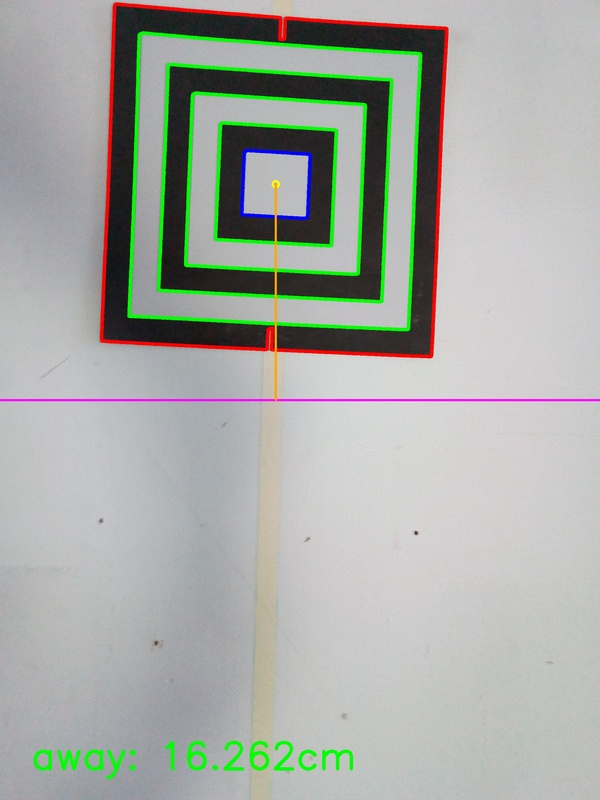
\includegraphics[width=0.95\linewidth]{pics/zielfeld/05.jpg}
        \caption{sämtliche Quadrate}
        \label{fig:zielfeld5}
    \end{subfigure}
    \begin{subfigure}{0.3\textwidth}
        \centering
        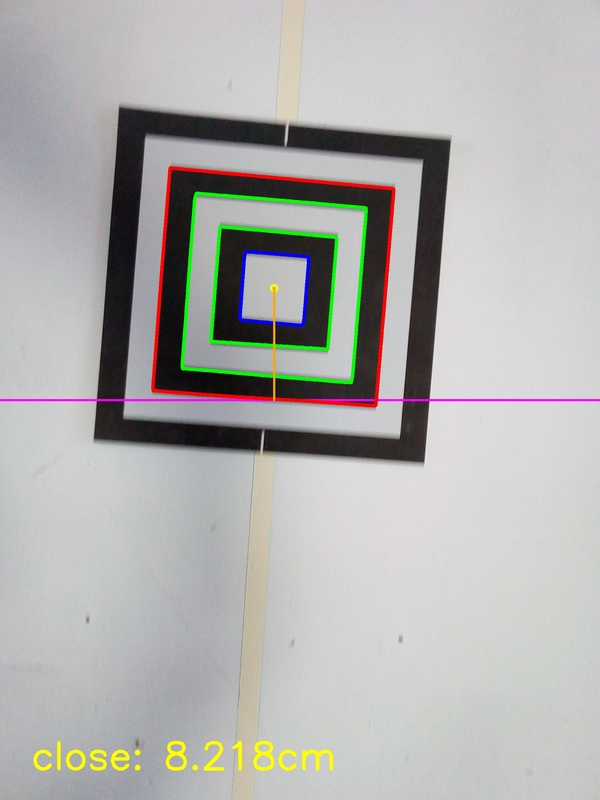
\includegraphics[width=0.95\linewidth]{pics/zielfeld/06.jpg}
        \caption{verschwommene Aufnahme}
        \label{fig:zielfeld6}
    \end{subfigure}
    \vskip\baselineskip
    \begin{subfigure}{0.3\textwidth}
        \centering
        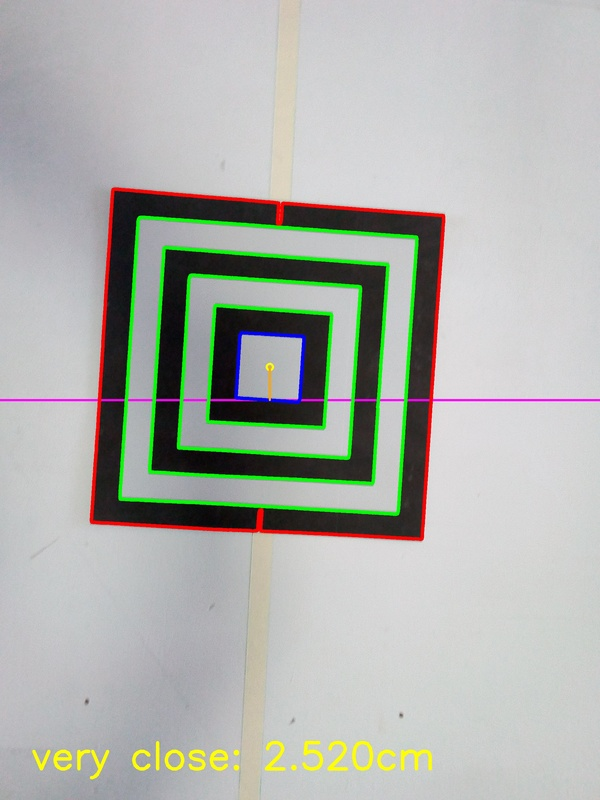
\includegraphics[width=0.95\linewidth]{pics/zielfeld/07.jpg}
        \caption{immer näher}
        \label{fig:zielfeld7}
    \end{subfigure}
    \begin{subfigure}{0.3\textwidth}
        \centering
        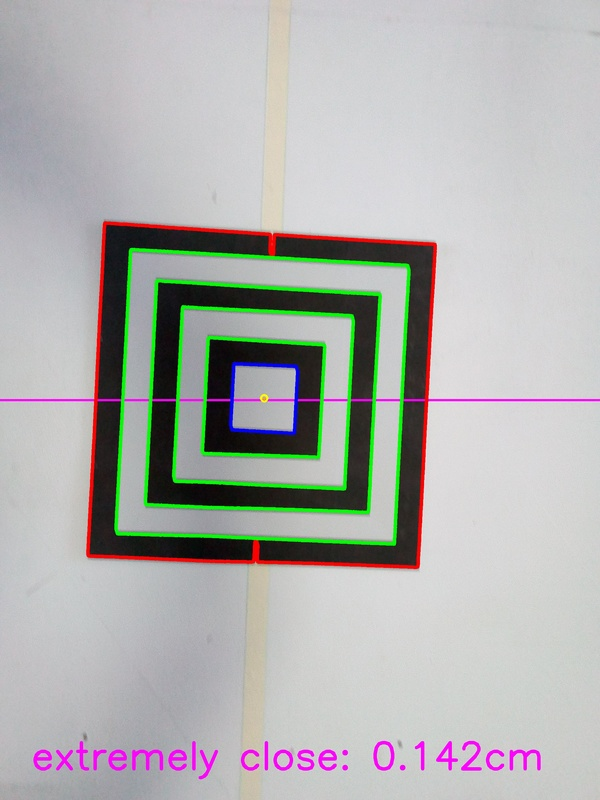
\includegraphics[width=0.95\linewidth]{pics/zielfeld/08.jpg}
        \caption{extrem nahe}
        \label{fig:zielfeld8}
    \end{subfigure}
    \begin{subfigure}{0.3\textwidth}
        \centering
        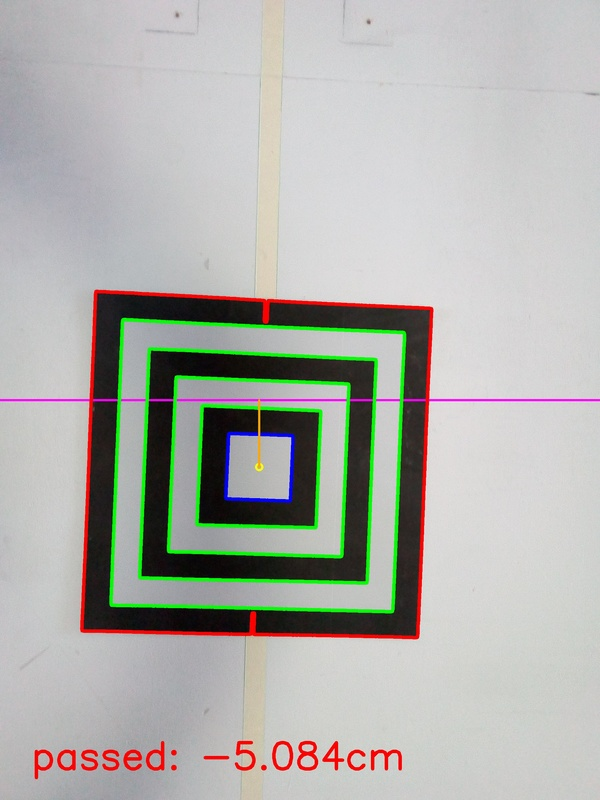
\includegraphics[width=0.95\linewidth]{pics/zielfeld/09.jpg}
        \caption{vorbei}
        \label{fig:zielfeld9}
    \end{subfigure}
    \label{fig:bildserie}
    \caption{Die Bildserie zeigt das Überfahren des Zielfeldes aus Kameraperspektive.}
\end{figure}

\subsection{Auflösung und Verarbeitungsgeschwindigkeit}

Das verwendete Kameramodul \cite{picam} unterstützt eine Bildauflösung von bis zu $3280\times2464$ Bildpunkten, was acht Megapixeln entspricht. Bei den Tests wurden verschiedene Auflösungen ausprobiert, etwa HD-Auflösung ($1080\times1920$ Pixel).\footnote{Die Orientierung der Kamera wird über die Auflösung der Form $\text{Breite}\times\text{Höhe}$ angegeben. Die Auflösung $1920\times1080$ entspricht der HD-Auflösung in \textit{Landscape}-Orientierung (Breitbild), die Auflösung $1080\times1920$ entspricht der HD-Auflösung in \textit{Portrait}-Orientierung (Hochformat). Da das Blickfeld der Kamera möglichst weit nach vorne und nicht in die Breite reichen soll, wird das Hochformat verwendet.} Die besten Ergebnisse wurden mit einer Auflösung von $480\times640$ (VGA-Auflösung) erreicht. Diese geringe Auflösung hat folgende Vorteile:

\begin{description}
    \item[Performance] Das Auswerten von Bildern in HD-Auflösung dauerte ca. $550$ Millisekunden. Mit VGA-Auflösung konnten Bilder in durchschnittlich $45$ Millisekunden ausgewertet werden. Das entspricht einem Performancegewinn von ca. Faktor $12$.
    \item[Unschärfe] Bei der vorliegenden Aufgabe hat sich eine gewisse Unschärfe bei den aufgenommenen Bildern als vorteilhaft erwiesen, da kleinere Konturen, wie etwa Verschmutzungen auf dem Zielfeld und Klebestreifenrückstände auf der Unterlage, bereits bei der Bildaufnahme verschwimmen und so nicht als Konturen erkannt werden. Die scharfen Konturen des Zielfeldes waren bei den Aufnahmen aber dennoch genug scharf.
\end{description}

Für die Testdurchläufe wurden die aufgenommenen Bilder zur späteren Auswertung jeweils abgespeichert. Das Abspeichern der Bilder nahm jeweils ungefähr die Hälfte der Bildverarbeitungszeit in Anspruch: Dauerte die Verarbeitung eines Bildes $45$ Millisekunden, benötigte die Abspeicherung weitere $20$ Millisekunden. Für den Wettbewerb wird das Abspeichern der Bilder aus Performancegründen deaktiviert.
